% !TeX root = RJwrapper.tex
\title{Monte-Carlo Methods for Prediction Functions}
\author{by Zachary M. Jones}

\maketitle

\abstract{
An abstract of less than 150 words.
}

Many methods for estimating prediction functions produce estimated functions which are not directly human-interpretable because of their complexity: they may include high-dimensional interactions and/or complex nonlinearities. While a learning method's capacity to automatically learn interactions and nonlinearities is attractive when the goal is prediction, there are many cases where users want good predictions \textit{and} the ability to understand how predictions depend on the features. \code{mmpf} implements general methods for interpreting prediction functions using Monte-Carlo methods. These methods allow any function which generates predictions to be be interpreted. \code{mmpf} is currently used in other packages for machine learning like \code{edarf} and \code{mlr} \citep{jones2016,JMLR:v17:15-066}.

\section{Marginalizing Prediction Functions}

The core function of \code{mmpf}, \code{marginalPrediction}, allows marginalization of a prediction function so that it depends on a subset of the features. Say the matrix of features $\mathbf{X}$ is partitioned into two subsets, $\mathbf{X}_u$ and $\mathbf{X}_{-u}$, where the former is of primary interest. A prediction function $f$ which in the regression case maps $\mathbf{X} \rightarrow \mathbf{y}$, where $\mathbf{y}$ is a real-valued vector, can be estimated from $(\mathbf{X}, \mathbf{y})$ giving $\hat{f}$, which might not be additive or linear in the columns of $\mathbf{X}_u$, making $\hat{f}$ difficult to interpret directly. If we knew the joint distribution $\mathbb{P}(\mathbf{X}, \mathbf{y})$ and $f$ we could marginalze the joint distribution so that it only depends on $\mathbf{X}_u$, which would give us $f_u$, which only depends on a subset of the features $\mathbf{X}_u$.

$$f_u (\mathbf{X}_u) = \int f(\mathbf{X}_u, \mathbf{X}_{-u}) \mathbb{P}(\mathbf{X}) d \mathbf{X_{-u}}$$

However, we instead have $\hat{f}$ and also generally don't know the joint distribution of $(\mathbf{X}, \mathbf{y})$. To approximate $f_u$ we utiltize $\hat{f}$ as a plug-in estimator for $f$, and we assume that $\mathbb{P}(\mathbf{X}, \mathbf{y}) = \mathbb{P}(\mathbf{X}_{u}, \mathbf{y}) \mathbb{P}(\mathbf{X}_{-u}, \mathbf{y})$, which allows us to compute

$$\hat{f}_{u}(\mathb{X}_{u}) = \int \hat{f}(\mathbf{X}_{u}, \mathbf{X}_{-u}) \mathbb{P}(\mathbf{X}_{-u}) d \mathbf{X}_{-u}$$

which relies only on knowing the marginal distribution of $\mathbf{X}_{-u}$, which we can approximate using the empirical marginal distribution of $\mathbf{X}_{-u}$. 

This has the advantage of recovering the shape or functional form of of $\hat{f}_u$ \textit{if} the joint probability of $\mathbf{X}$ can be factorized to be additive or multiplicative in $(\mathbf{X}_u, \mathbf{X}_{-u})$ \citep{friedman2001greedy}.

These assumptions imply the following Monte-Carlo integration procedure

$$\hat{f}_u (\mathbf{X}_u) = \sum_{i = 1}^N \hat{f} (\mathbf{X}_u, \mathbf{X}_{-u}^{(i)})$$

Partial dependence is the result of this type of procedure; it is the expected value of the marginalized prediction function $\hat{f}_u$ evaluated at values of $\mathbf{X}_u$ \cite{friedman2001greedy}. \code{marginalPrediction} allows users to compute partial dependence and any other function of this marginalized function easily.

\begin{example}
  library(mmpf)
  library(randomForest)
  
  data(iris)
  fit = randomForest(Species ~ ., data = iris)

  mp = marginalPrediction(data = iris[, -ncol(iris)],
    vars = "Petal.Width",
    n = c(10, nrow(iris)), model = fit, uniform = TRUE,
    predict.fun = function(object, newdata) predict(object, newdata, type = "prob"))
  print(mp)
  ##     Petal.Width    setosa versicolor virginica
  ##  1:   0.1000000 0.6374133  0.2337733 0.1288133
  ##  2:   0.3666667 0.6374133  0.2337733 0.1288133
  ##  3:   0.6333333 0.6356267  0.2350533 0.1293200
  ##  4:   0.9000000 0.1707200  0.5997333 0.2295467
  ##  5:   1.1666667 0.1688267  0.6016267 0.2295467
  ##  6:   1.4333333 0.1688133  0.5880800 0.2431067
  ##  7:   1.7000000 0.1640400  0.4242800 0.4116800
  ##  8:   1.9666667 0.1619867  0.2066667 0.6313467
  ##  9:   2.2333333 0.1619867  0.2047867 0.6332267
  ## 10:   2.5000000 0.1619867  0.2047867 0.6332267
\end{example}

If the prediction function is marginalized so that it depends on a low dimensional subset of the features, for example one or two dimensions, then it can be easily visualized, as in Figure \ref{figure:mp}.

\begin{figure}
  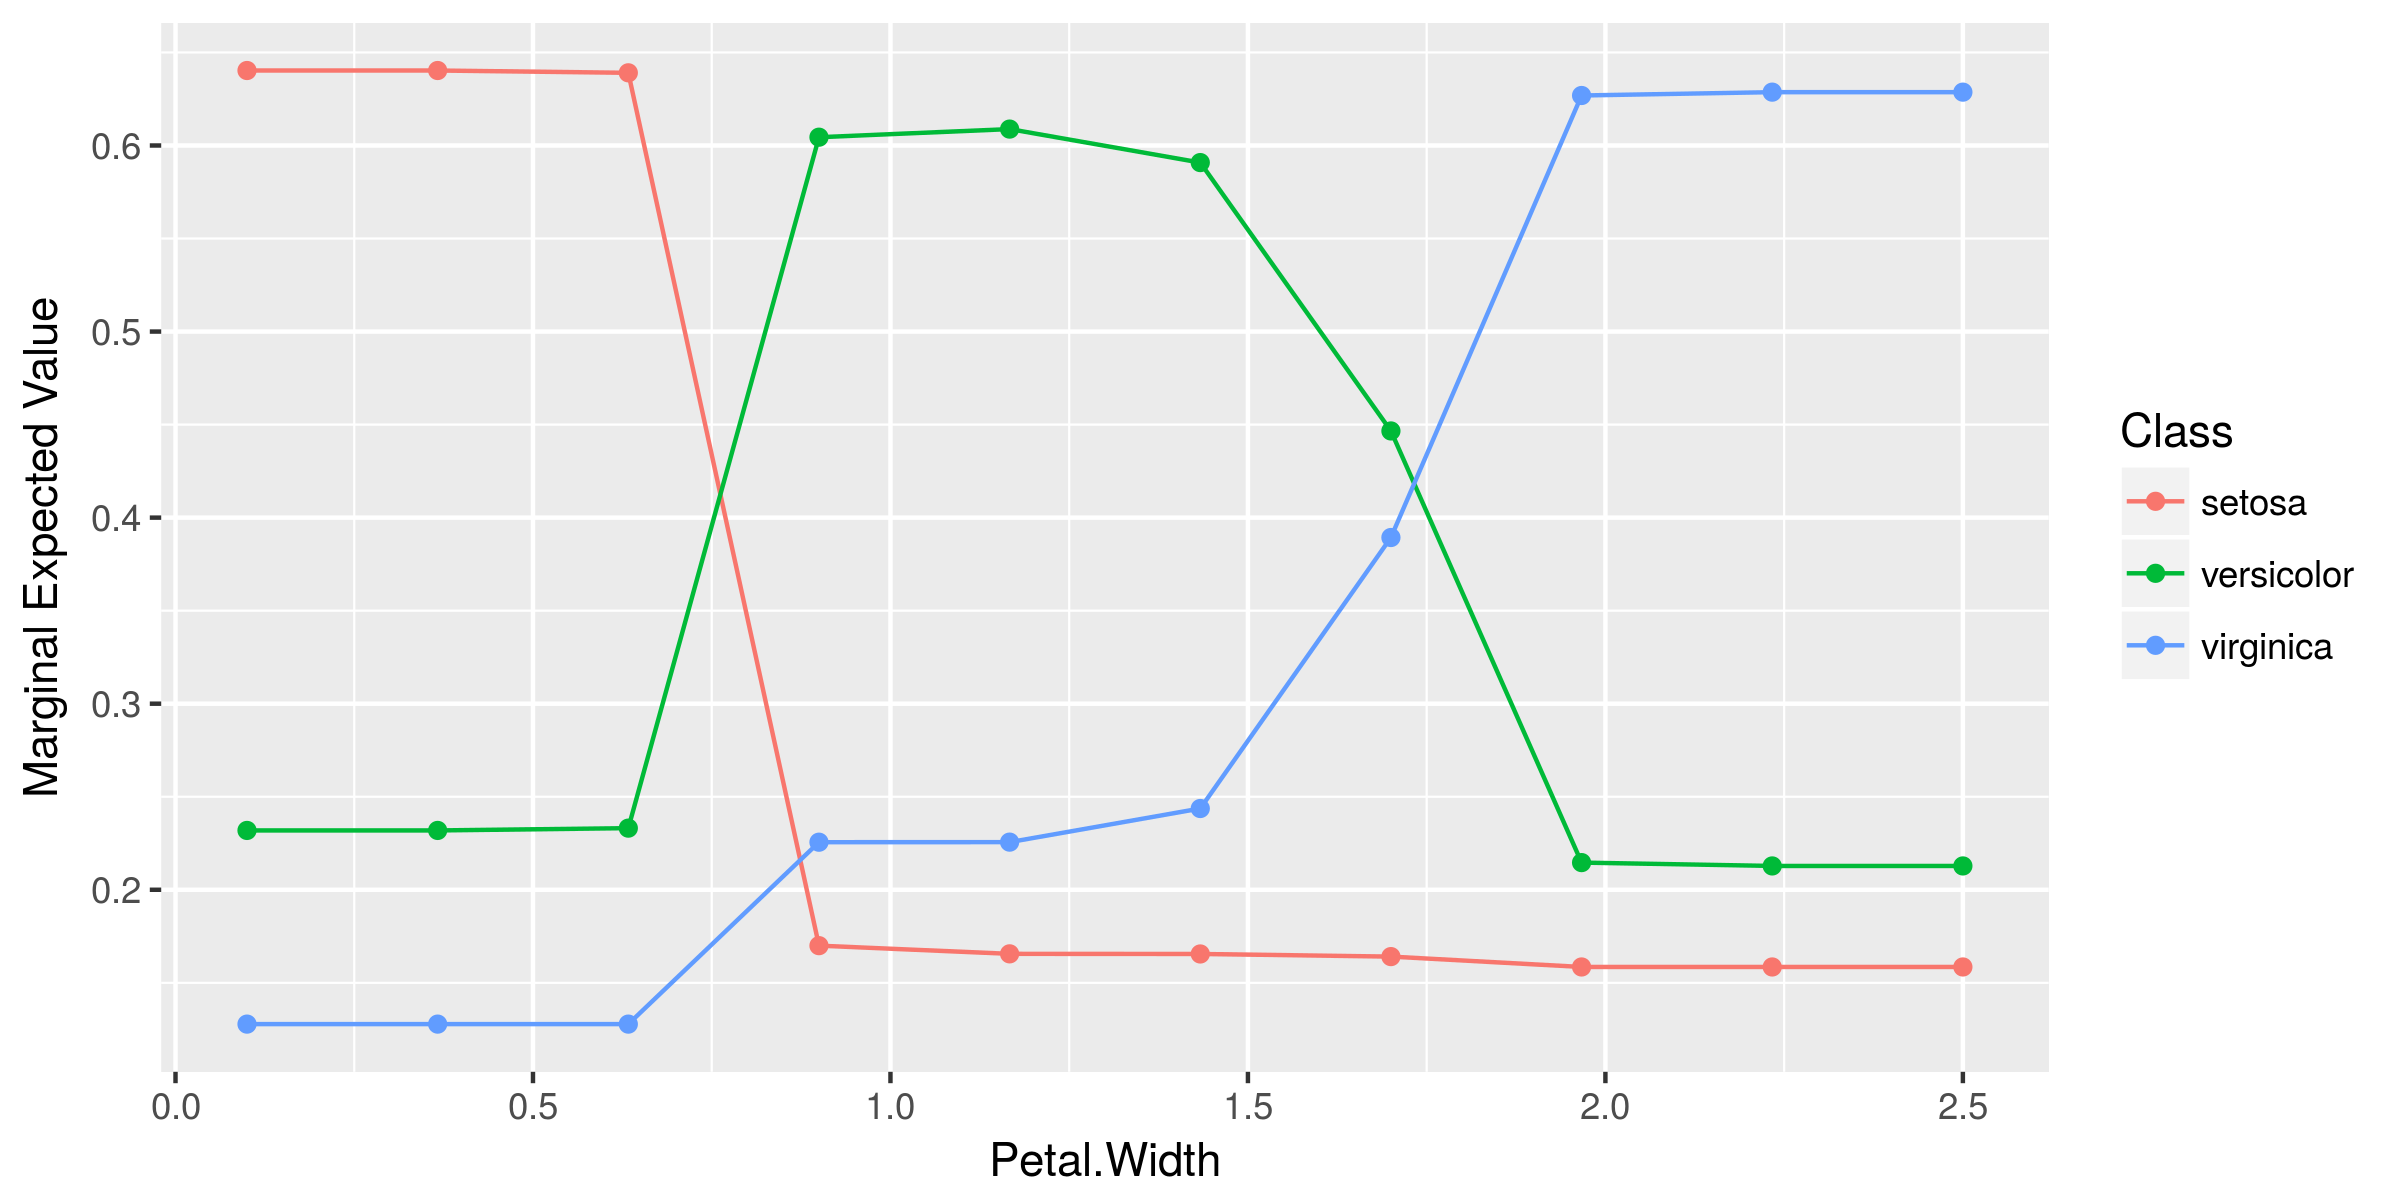
\includegraphics[width=\textwidth]{mp.png}
  \caption{The expected value of $\hat{f}$ estimated by a random forest and marginalized by Monte-Carlo integration to depend only on ``Petal.Width.'' \label{figure:mp}}
\end{figure}

As mentioned earlier, \textit{any} function of the marginalized function can be computed, including vector-valued functions. For example the expectation and variance of the marginalized function can be simultaneously computed, the results of which are shown in Figures \ref{figure:mp_int_mean} and \ref{figure:mp_int_var}. Computing the variance of a marginalized function can be used for detecting interactions between $\mathbf{X}_u$ and $\mathbf{X}_{-u}$ \citep{goldstein2015peeking}.

\begin{example}
mp.int = marginalPrediction(data = iris.features,
  vars = c("Petal.Width", "Petal.Length"),
  n = c(10, nrow(iris)), model = fit, uniform = TRUE,
  predict.fun = function(object, newdata) predict(object, newdata, type = "prob"),
  aggregate.fun = function(x) list("mean" = mean(x), "variance" = var(x)))
\end{example}

\begin{figure}
  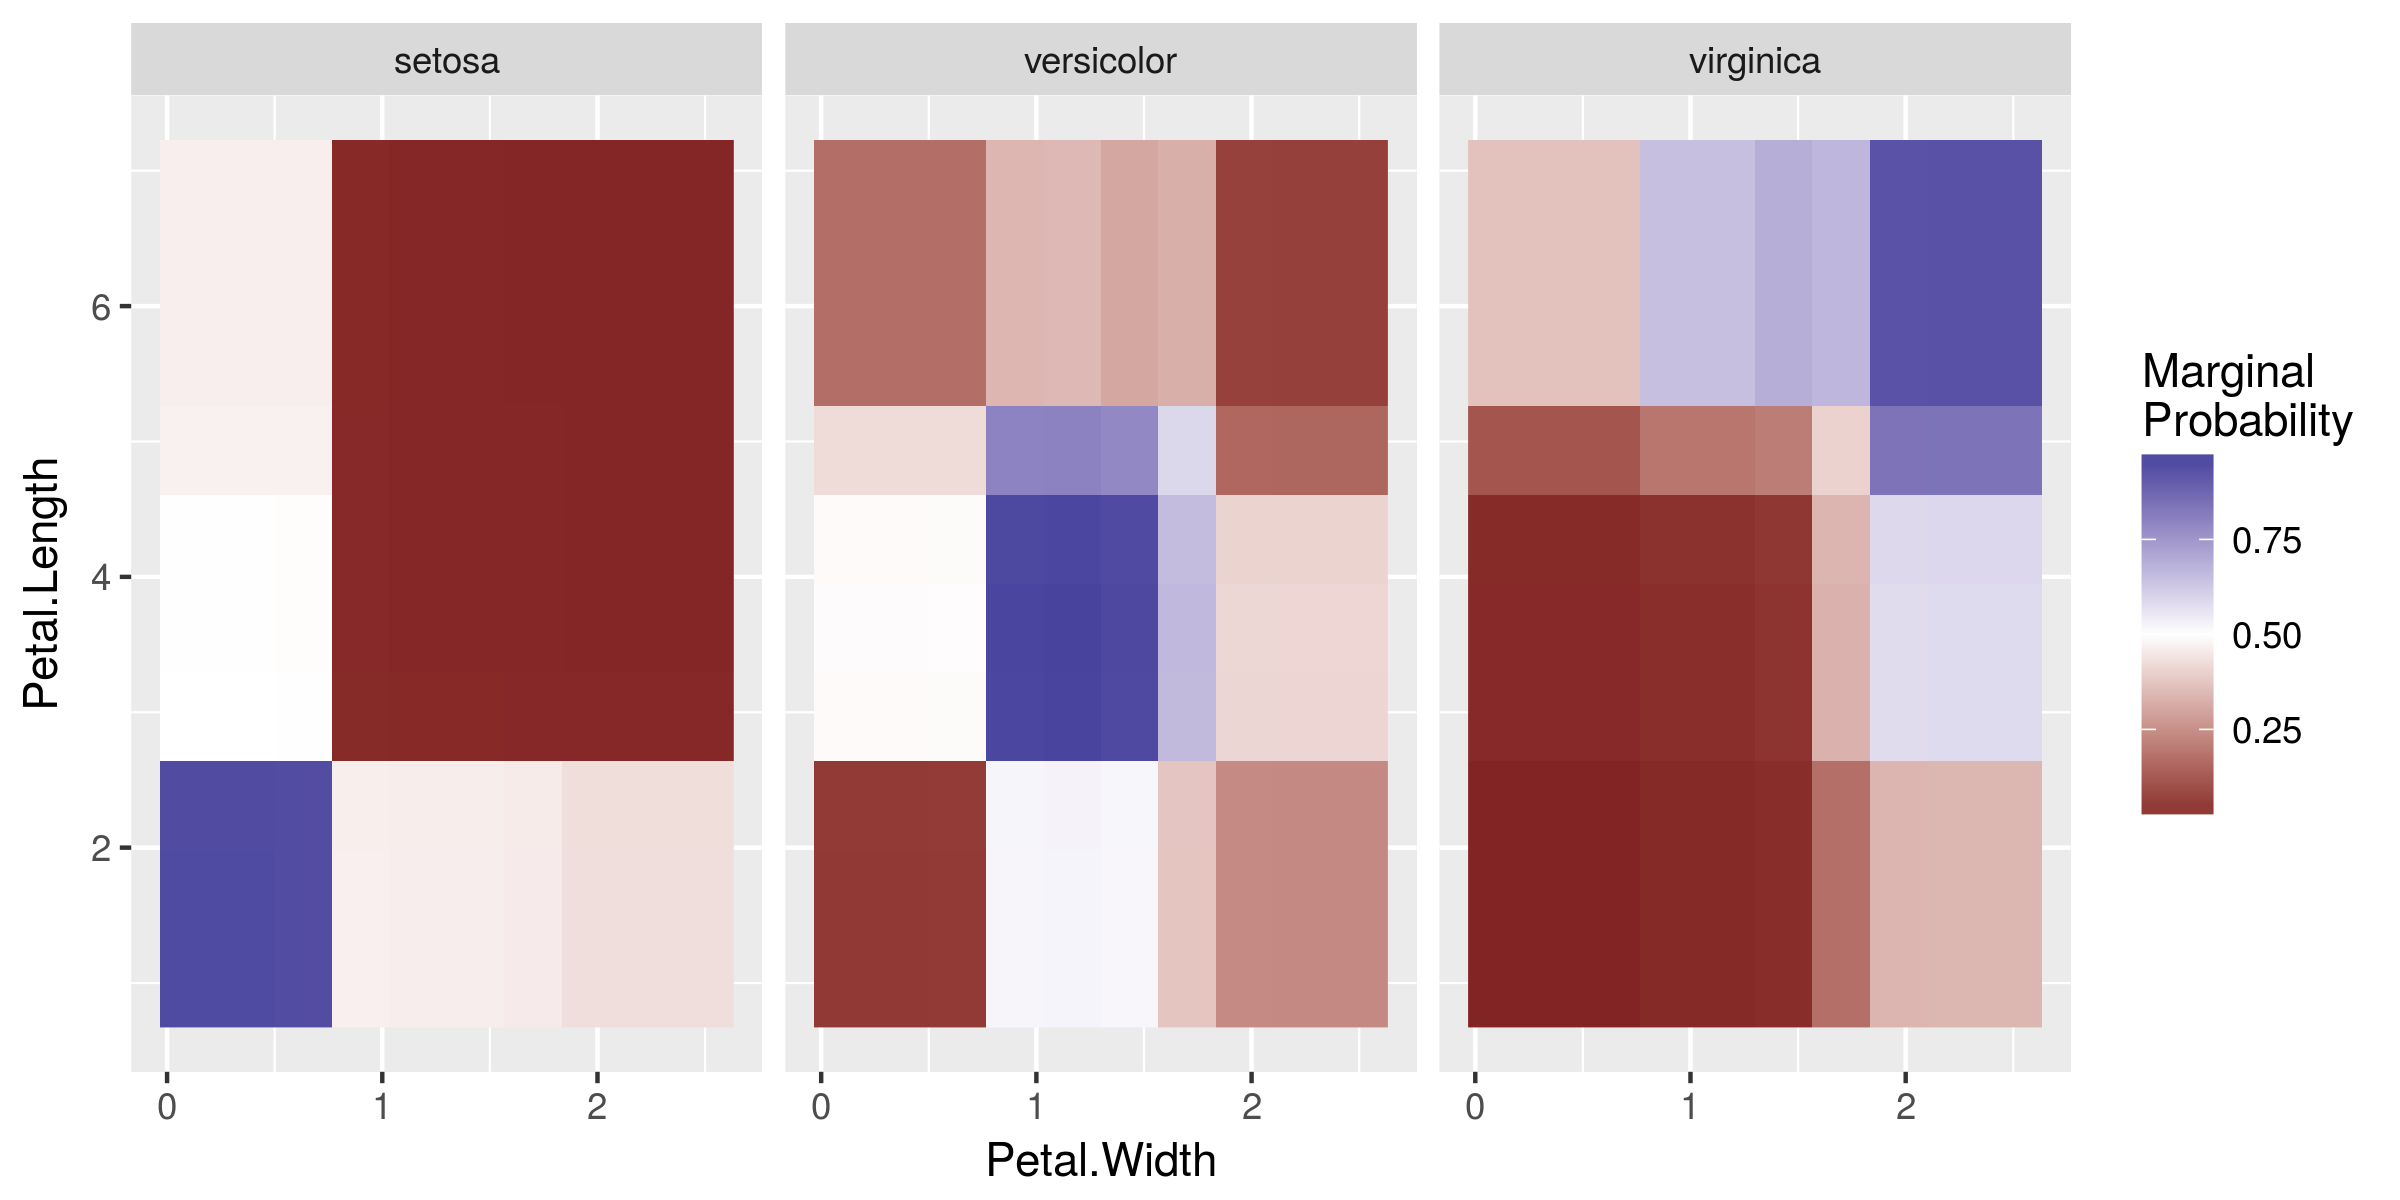
\includegraphics[width=\textwidth]{mp_int_mean.png}
  \caption{The expected value of $\hat{f}$ estimated by a random forest and marginalized by Monte-Carlo integration to depend only on ``Petal.Width'' and ``Petal.Length.'' \label{figure:mp_int_mean}}
\end{figure}

\begin{figure}
  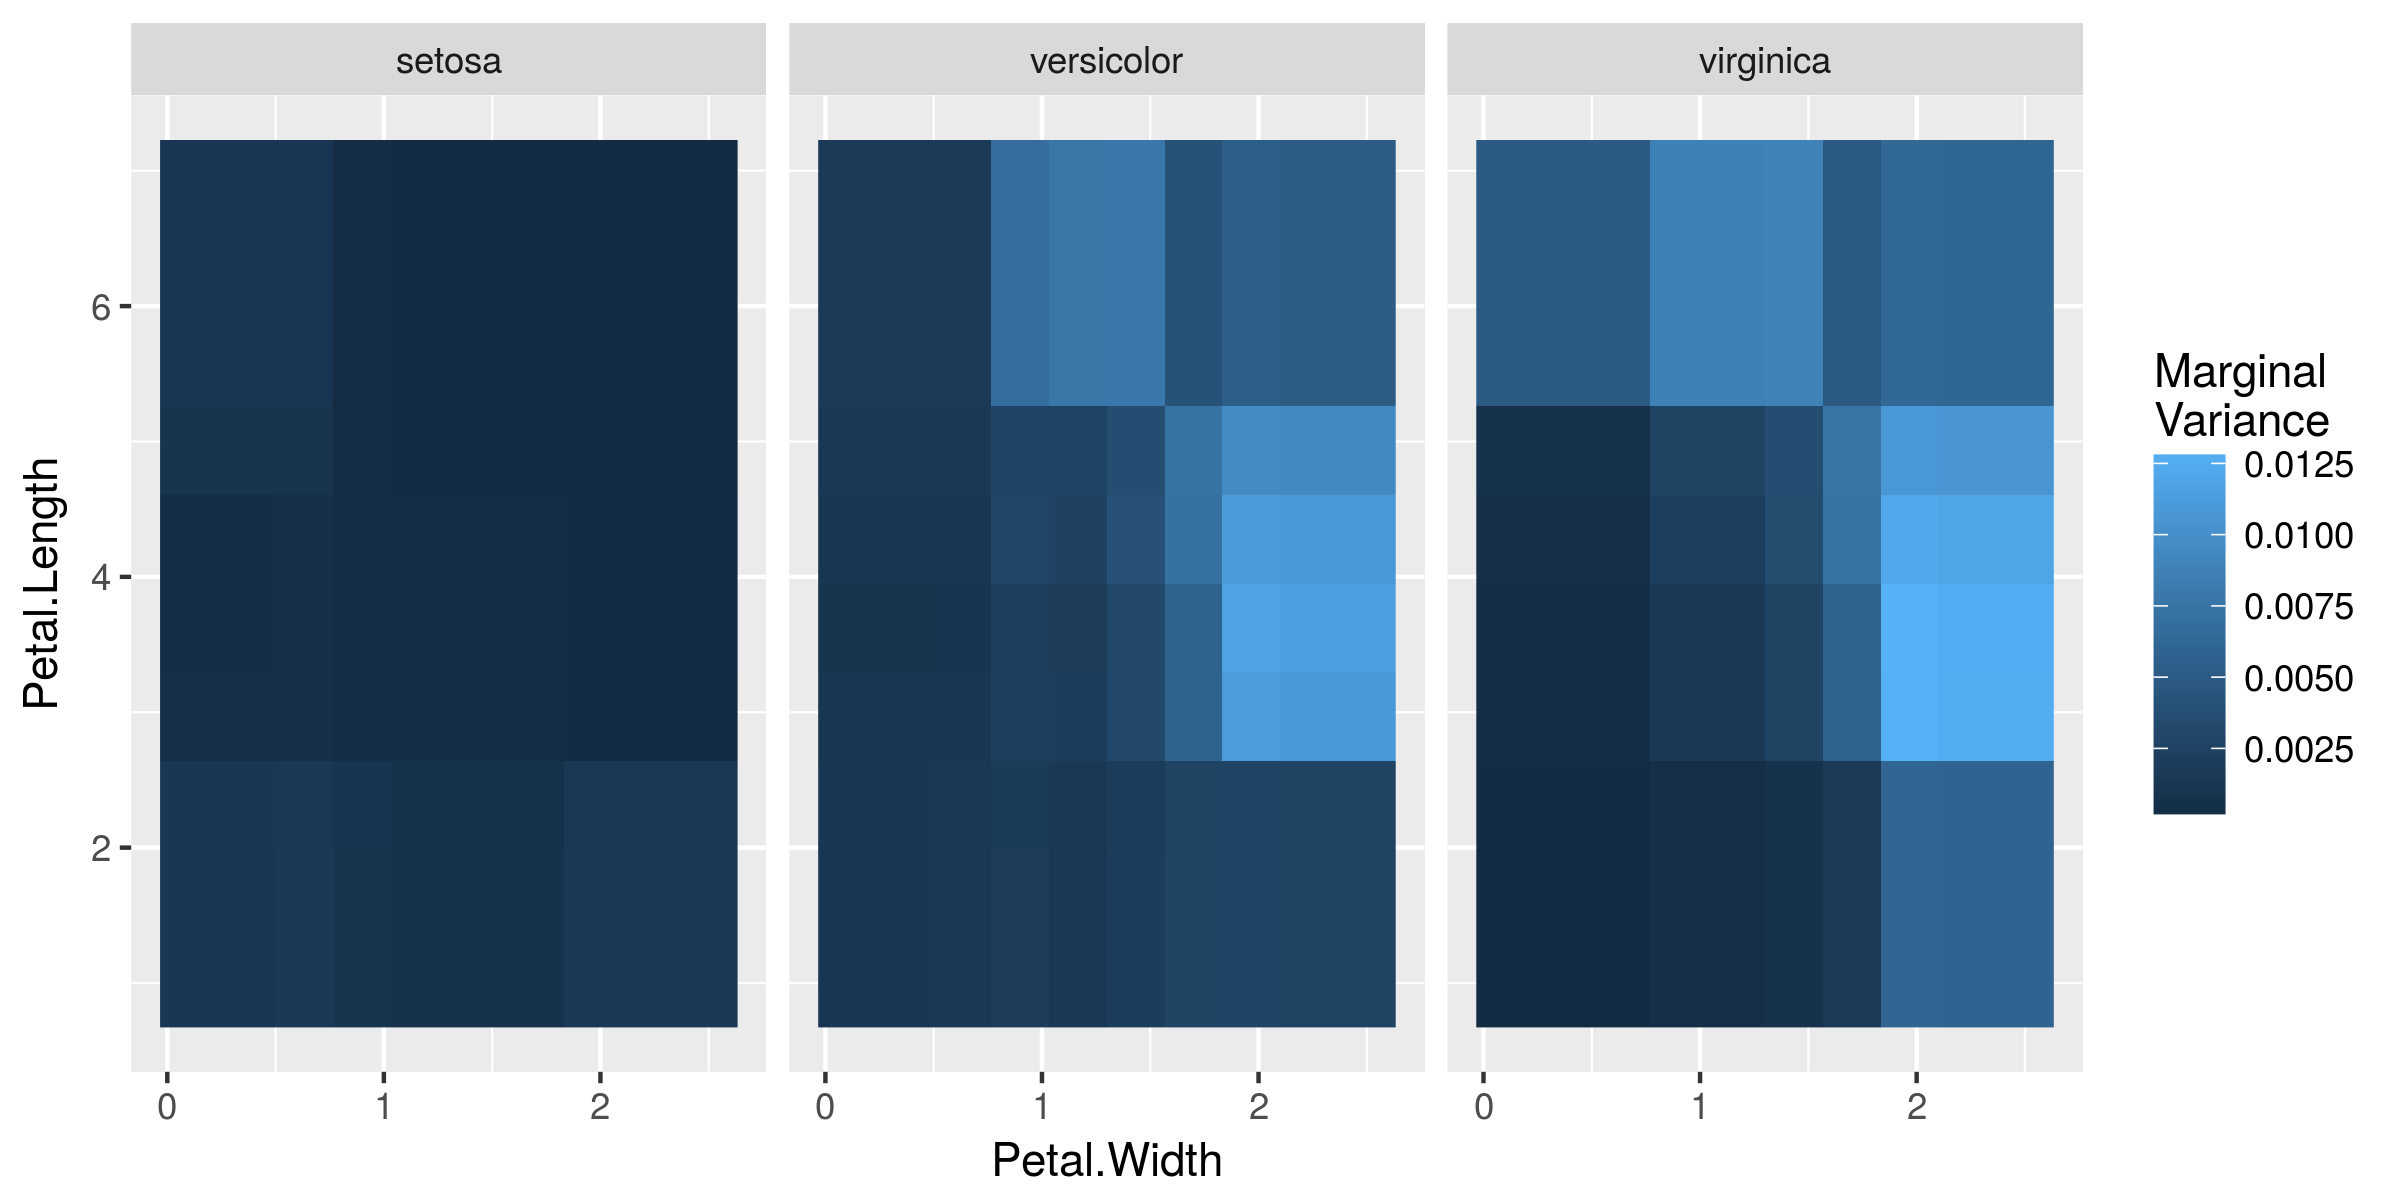
\includegraphics[width=\textwidth]{mp_int_var.png}
  \caption{The variance of $\hat{f}$ estimated by a random forest and marginalized by Monte-Carlo integration to depend only on ``Petal.Width'' and ``Petal.Length.'' Non-constant variance indicates interaction between these variables and those marginalized out of $\hat{f}$. \label{figure:mp_int_var}}
\end{figure}

\code{marginalPrediction} can also perform Monte-Carlo integration against probability measures which are functions of the training data. This can help avoid problems from the assumption that the joint distribution of $\mathbf{X}$ is a product distribution. When $\mathbb{P}(\mathbf{X}) \neq \mathbb{P}(\mathbf{X}_u)\mathbb{P}(\mathbf{X}_{-u})$ assuming that this is the case can result in evaluating in a $\hat{f}_u$ which is constructed from model behavior in regions of the of the feature space which occur with low probability under $\mathbb{P}(\mathbf{X})$, making $\hat{f}_u$ depend heavily on the behavior of the method used to learn $\hat{f}$ in regions of little or no data \citep{hooker2012generalized}.

As a simple example consider the case of data from a deterministic function which is linear across its support. Specifically, $\mathbf{y} = f(\mathbf{X}) = \mathbf{X} \mathbf{w}$ where $\mathbf{X}$ is a two dimensional matrix of features each of which is drawn from an independent uniform distribution on ${0, 1}$ and $\mathbf{w}$ is a vector of real-valued weights.

Suppose that there is an outlier which is extreme in both $X_1$ and $y$, but perfectly normal in $X_2$: $X_1 = 1.5$, $X_2 = .5$, and, $y = X_1^2 + X_2$. Figure \ref{figure:mp_w_data} shows the empirical distribution of $\mathbf{X}$. Some methods for constructing $\hat{f}$ will strongly depend on this outlying point, as is the case in this example. Using support vector regression and a polynomial kernel results in dramatic nonlinearity when $X_1 > 1$. If we compute unweighted partial dependence assume a discrete uniform distribution on $X_1$, which includes the outlying point at $X_1 = 1.5$.

Although this outlier is easy to see, because this problem is low-dimensional, in a higher dimensional space outliers are difficult to detect visually. In these cases Monte-Carlo methods for interpreting $\hat{f}$ will also depend heavily on these sorts of points. Constructing a weight function, which takes points of the same dimension as $\mathbf{X}$ and outputs a scalar which encodes some notion of ``closeness'' to the training data can help alleviate this problem, as shown in Figure \ref{figure:mp_w}. 


\begin{figure}
  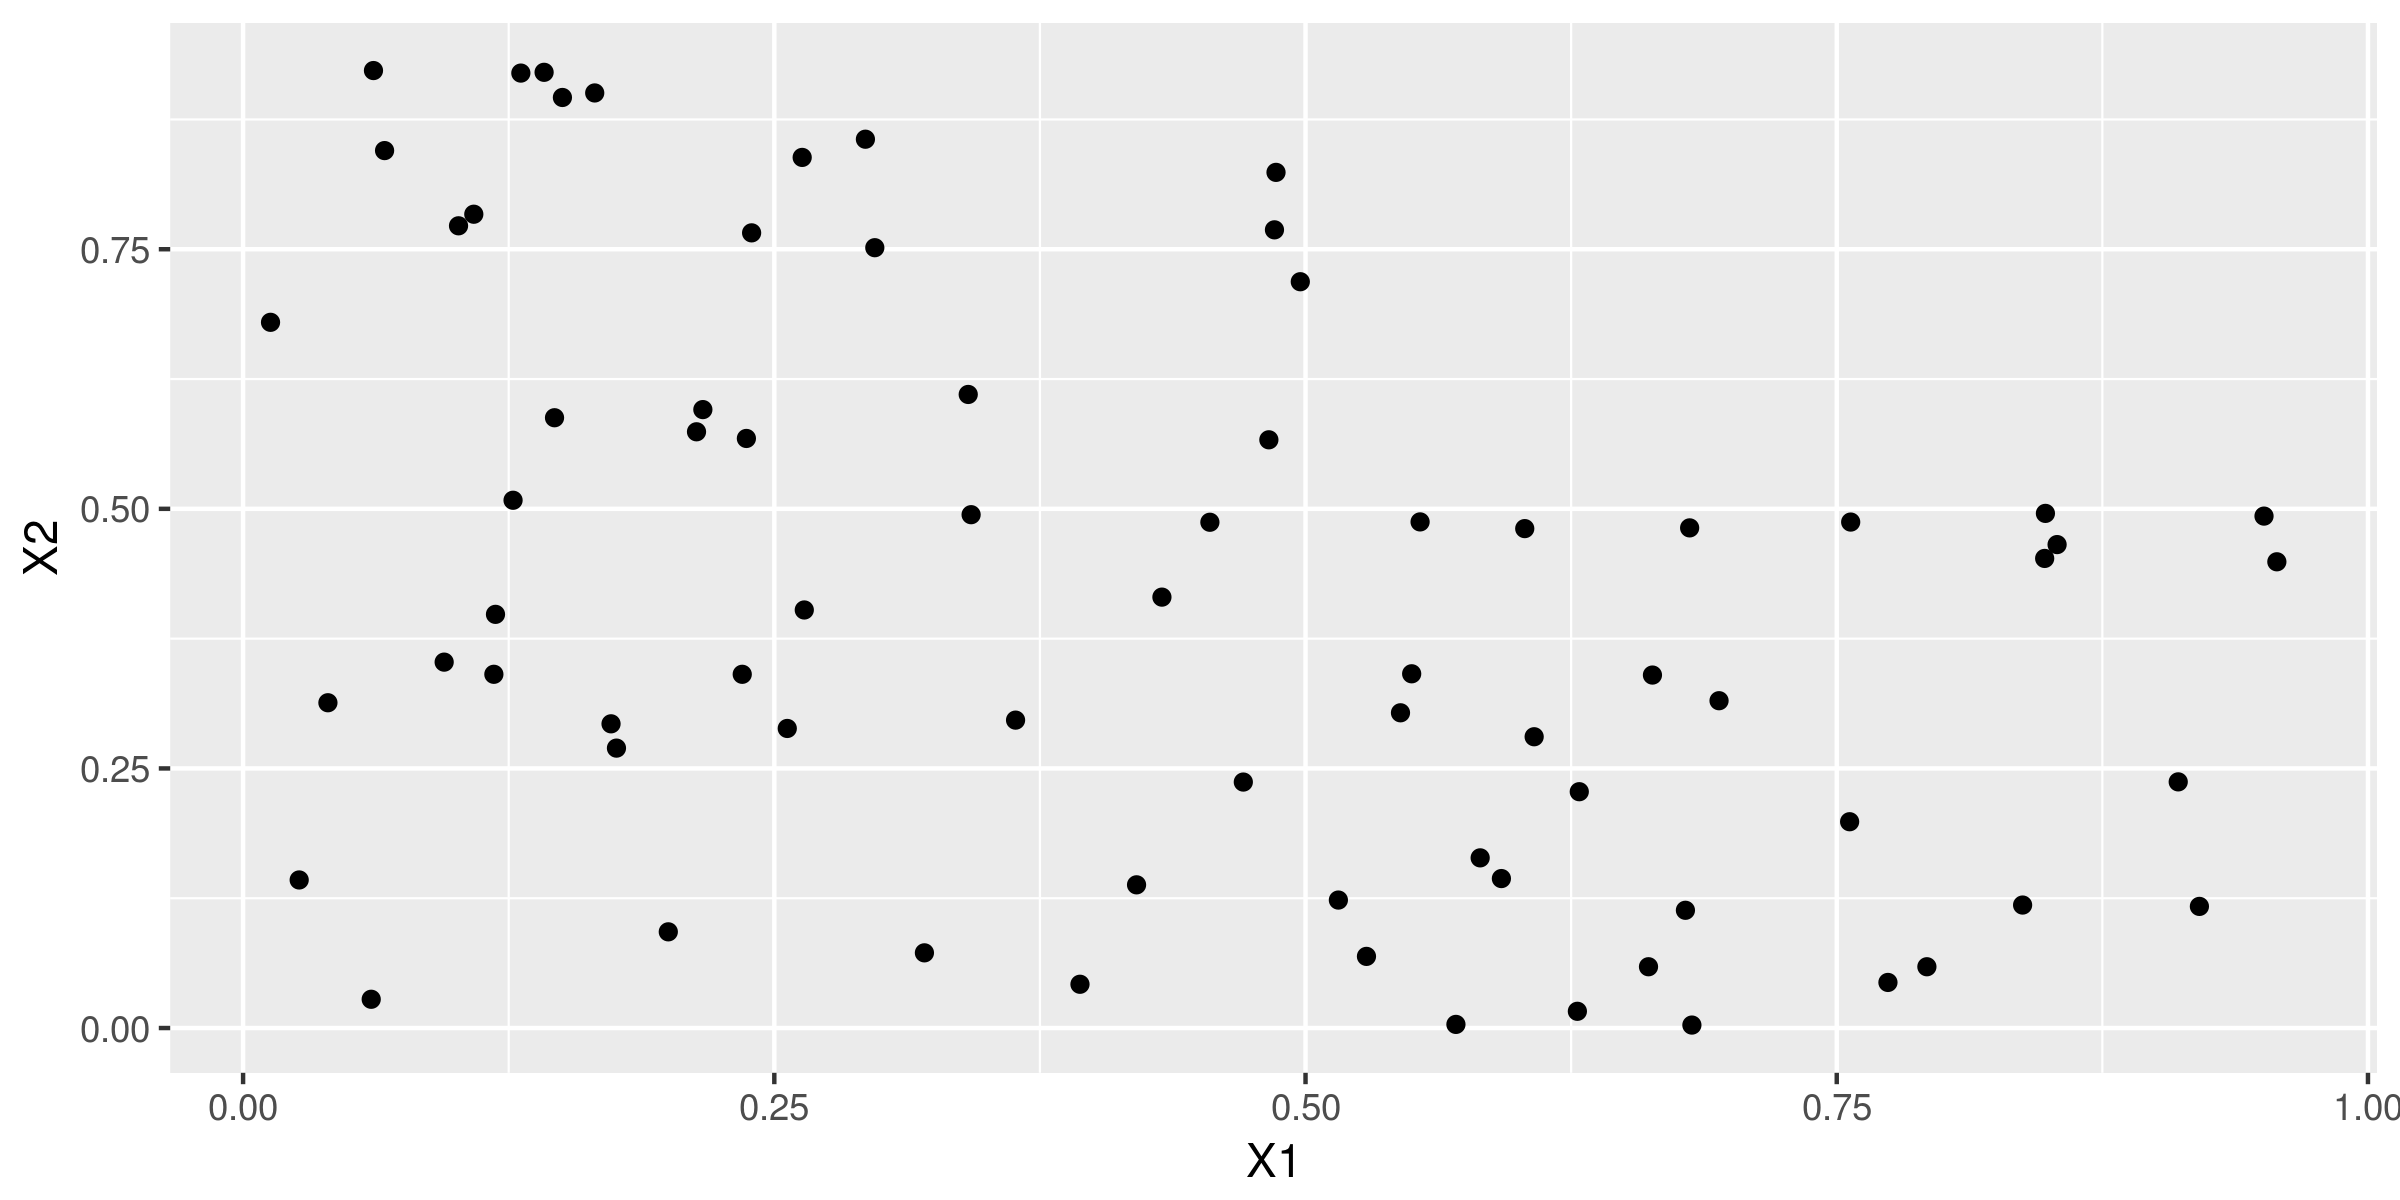
\includegraphics[width=\textwidth]{mp_w_data.png}
  \caption{The joint distribution of the features, both of which are independent uniform draws, with the except of one point at $X_1 = 1.5, X_2 = .5$, which lies outside the support and is an outlier.\label{figure:mp_w_data}}
\end{figure}

\begin{figure}
  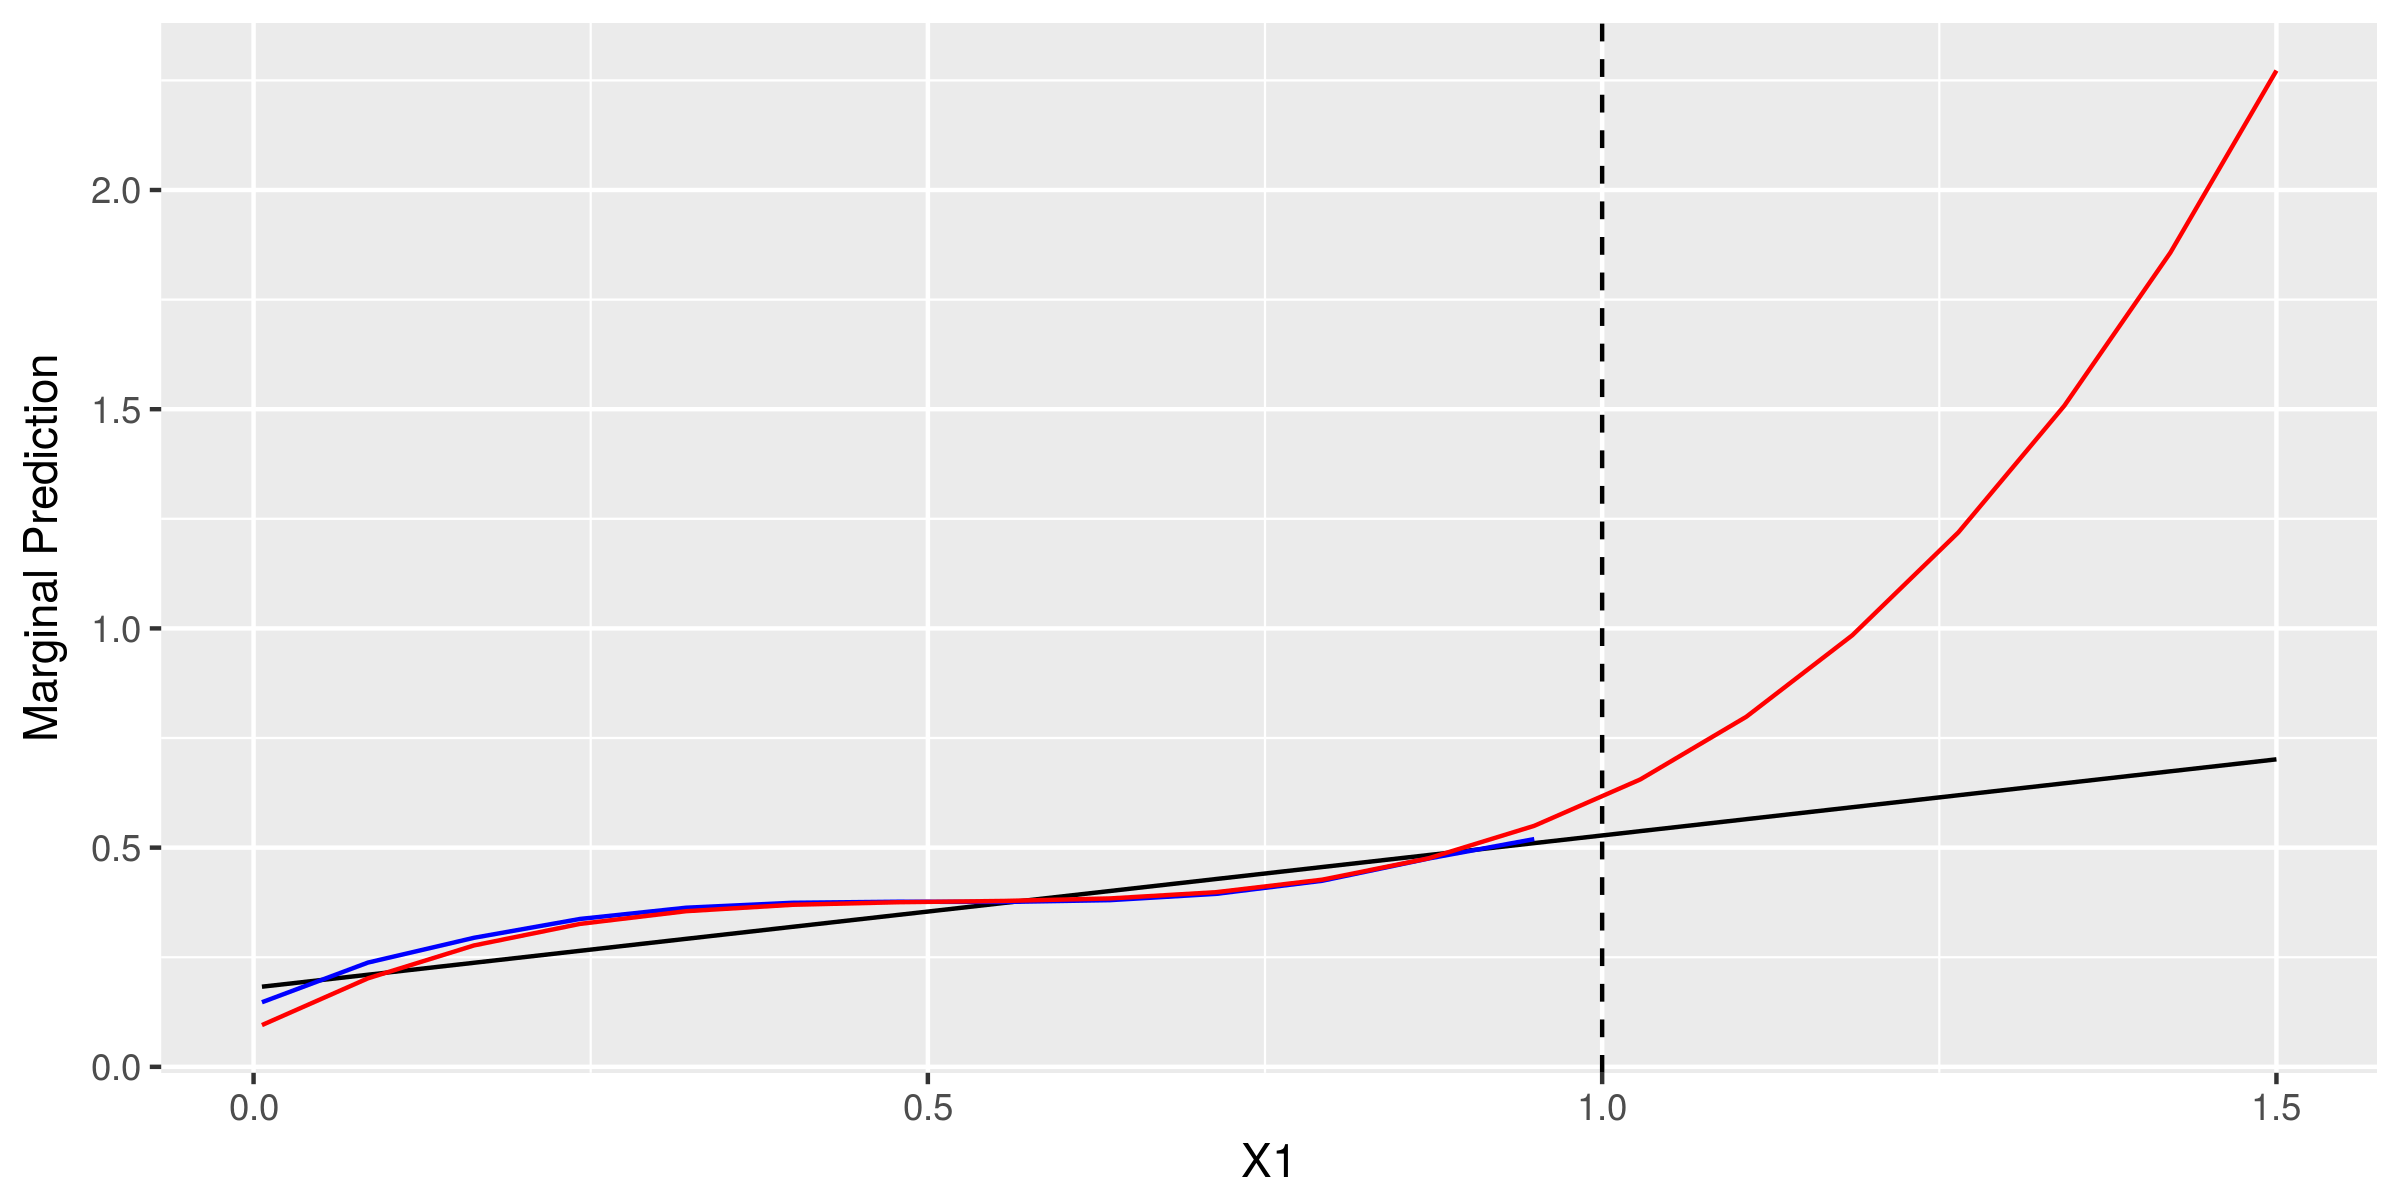
\includegraphics[width=\textwidth]{mp_w.png}
  \caption{$\hat{f}$ marginalized to depend only on $\mathbf{X}_1$ without weighting, shown in red, or with weighting based on Tukey's half-space depth, shown in blue. The true marginal relationship is shown in black and the dashed line shows the true bounds of the support of $X_1$. \label{figure:mp_w}}
\end{figure}

With observed outlying points model behavior can be controlled by choosing a loss function which does not heavily weight outlying points. However, this is not always possible or desirable. Outliers can also be generated by the aforementioned product distribution assumption. This can be especially problematic when features are highly correlated, making their joint distribution far from uniform.





\bibliography{RJreferences}

\address{Zachary M. Jones\\
  Pennsylvania State University\\
  University Park, Pennsylvania\\
  United States\\}
\email{zmj@zmjones.com}